\documentclass[11pt]{article}
\usepackage[a4paper,margin=2.4cm]{geometry}
\usepackage{amsmath,amssymb}
\usepackage{graphicx}
\usepackage{booktabs}
\usepackage{array}
\usepackage{longtable}
\usepackage{xcolor}
\usepackage[hidelinks]{hyperref}
\usepackage{caption}
\captionsetup{font=small}

\newcommand{\Ombg}{h^2\Omega_{\rm GW}}
\newcommand{\gD}{g_D}
\newcommand{\mAp}{m_{A'}}
\newcommand{\mrho}{m_\rho}
\newcommand{\betaH}{\beta/H}

\title{\textbf{Gravitational waves from a classically scale-invariant dark $U(1)_D$
first-order phase transition and their confrontation with pulsar-timing-array data}}
\author{DarkAgents}
\date{2026-06-09}

\begin{document}
\maketitle

\begin{abstract}
We report an end-to-end \texttt{fopt-pta} pipeline analysis of a classically
scale-invariant (conformal) dark $U(1)_D$ extension of the Standard Model (SM),
in which a complex scalar $\Phi$ and a dark gauge boson $A'$ undergo
Coleman--Weinberg (CW) radiative symmetry breaking. We compute the stochastic
gravitational-wave background (SGWB) from the resulting strongly supercooled
first-order phase transition (FOPT), confront the spectrum with the NANOGrav
15-year (NG15) dataset through a PTArcade Bayesian inference campaign, and audit
the laboratory, astrophysical and cosmological constraints on the preferred
region, together with the dominant modelling assumptions. The campaign favours
a dark vacuum expectation value (vev) $v\simeq1.09$~GeV and gauge coupling
$\gD\simeq0.528$ (MAP), corresponding to a GeV-scale dark photon. No constraint
currently excludes the $1\sigma$ region, but the preferred region is
\emph{provisional}: it rests on a no-supermassive-black-hole-binary (SMBHB)
foreground fit, an order-of-magnitude gauge-dependence theory uncertainty on
$\Ombg$, an unresolved $\xi=1$ versus $\epsilon\simeq0$ internal tension, and
four high-priority constraint calculations that remain to be performed.
\end{abstract}

\section{Prompt}
The verbatim user request was: \emph{``can you study the model in
\texttt{input/u1conformal/prompt.md}?''} The referenced specification describes a
classically scale-invariant/conformal dark $U(1)_D$ extension of the SM
(complex scalar $\Phi$ plus dark gauge boson $A'$, CW radiative breaking,
free parameters $v$ and $\gD$), and requests: (i)~analysis of the GW spectrum
from a FOPT and comparison to PTA data; (ii)~preparation of a PTArcade inference
campaign and extraction of the parameter-space region probeable by PTArcade;
(iii)~a check of all collider/astrophysical/cosmological constraints; and
(iv)~identification of assumptions, uncertainties and caveats relevant for
interpreting the results. The orchestrator ran the full \texttt{fopt-pta}
pipeline, skipped the \texttt{proposer-agent} (the model is self-contained), and
proceeded past the critic's non-blocking clarifications with standard
conformal-CW defaults.

\section{Model description (critic validation)}
\label{sec:model}
The dark-sector Lagrangian is
\begin{equation}
\mathcal{L}_D = |D_\mu\Phi|^2 - \lambda_\Phi|\Phi|^4
- \tfrac14 F'_{\mu\nu}F'^{\mu\nu},\qquad
D_\mu = \partial_\mu - i\gD A'_\mu ,
\end{equation}
with $\Phi(x)=(\chi+\rho(x)+iG(x))/\sqrt2$, where $\chi$ is the classical
background field, $\rho$ the radial mode (scalon) and $G$ the Goldstone mode
eaten by $A'$. The tree potential is $V_{\rm tree}(\chi)=\lambda_\Phi\chi^4/4$
with no tree-level mass term, so the theory is classically scale invariant;
scale invariance is broken radiatively (CW dimensional transmutation). The
field-dependent gauge-boson mass is $\mAp^2(\chi)=\gD^2\chi^2$, and the
radiatively generated radial mass is
\begin{equation}
\mrho^2=\beta_\lambda v^2,\qquad
\beta_\lambda=\frac{1}{8\pi^2}\Big(\sum_b n_b g_b^4-\sum_f n_f g_f^4\Big)
=\frac{3\gD^4}{8\pi^2},
\end{equation}
with the only contribution from the dark gauge boson ($n_b=3$, $g_b=\gD$).
The optional Higgs portal $\lambda_{H\Phi}|H|^2|\Phi|^2$ and kinetic mixing
$(\epsilon/2)F'_{\mu\nu}F^{\mu\nu}$ are assumed negligible for the PT/GW
dynamics. The dark and visible sectors are assumed thermalised at a common
temperature, $\xi\equiv T_{\rm dark}/T_{\rm vis}=1$, with the dark relativistic
degrees of freedom added to $g_*$.

The \texttt{critic-agent} validated the model with \emph{warning} status and
\emph{no red flags}. The independent (scanned) parameters are $\{v,\gD\}$; the
dependent quantities $\lambda_\Phi$ (CW-fixed by $V_{\rm eff}'(v)=0$),
$\mAp=\gD v$ and $\mrho=\sqrt{\beta_\lambda}\,v$ are computed internally by the
backend. The model matches the single-field scale-invariant selection rule of
\texttt{backend/semianalytic\_pipeline.py}. The critic raised five warnings and
three clarification requests, summarised in Table~\ref{tab:critic}.

\begin{table}[ht]
\centering\small
\caption{Critic warnings and clarification requests (source:
\texttt{handoff\_critique.json}).}
\label{tab:critic}
\begin{tabular}{p{0.30\textwidth} p{0.62\textwidth}}
\toprule
Item & Note \\
\midrule
$\lambda_\Phi$ meaning & Renormalized quartic at $\mu=v$ fixed by
$V_{\rm eff}'(v)=0$; no implicit tree mass term. \\
Thermal/Debye masses & Supplied by backend high-$T$ expansion
($\Pi_{A'}\sim(\gD^2/3)T^2$); no daisy resummation or RG running ($\mu=v$). \\
$\xi=1$ thermalization & Common-temperature assumption in mild tension with
negligible portal/kinetic mixing; affects $g_*$ and $N_{\rm eff}$. \\
Higgs portal & Must remain $\lambda_{H\Phi}\ll10^{-10}$ to preserve conformality. \\
Gauge dependence & Order-of-magnitude theory uncertainty on $\Ombg$
(arXiv:1707.06765); backend uses a fixed gauge. \\
\bottomrule
\end{tabular}
\end{table}

\section{Pipeline status}
\label{sec:status}
All pipeline stages produced schema-valid handoffs. Statuses are listed in
Table~\ref{tab:status}.

\begin{table}[ht]
\centering\small
\caption{Pipeline stage statuses.}
\label{tab:status}
\begin{tabular}{l l p{0.52\textwidth}}
\toprule
Stage & Status & Note \\
\midrule
preliminary-librarian & ok & 7 verified papers; model well-covered. \\
critic & warning & Validated, no red flags; 5 warnings, 3 clarifications. \\
fopt & ok & Backend executed; 148/157 viable, 8 failed, 1 not\_fopt. \\
pta & ok & Benchmark scan + PTArcade NG15 campaign ($10^5$ samples). \\
constraints & warning & No exclusions; 4 high-priority missing calculations. \\
prior-audit & warning & 22 items; high-severity uncontrolled items present. \\
\bottomrule
\end{tabular}
\end{table}

\section{Preliminary literature search}
\label{sec:lit}
The \texttt{preliminary-librarian-agent} identified seven verified papers
(Table~\ref{tab:lit}). The exact model (conformal dark $U(1)$ with complex
scalar plus dark gauge boson, CW breaking, supercooled FOPT, nHz GW matching
PTA) has been studied directly in
Gon\c{c}alves et al.~\cite{Goncalves2025} and Balan et al.~\cite{Balan2025};
the model structure and target band are therefore \emph{not} novel. The
remaining novelty lies in a dedicated, reproducible \texttt{fopt-pta}~+~PTArcade
Bayesian campaign for the minimal (DM-free) version with transparent FOPT
parameter extraction and gauge-uncertainty bookkeeping. Benchmark hints adopted
downstream: $\gD\in[0.55,0.9]$ and $v\sim0.1$--$0.7$~GeV (to land in the nHz
band), guided by the NANOGrav best-fit $\gD=0.59$ of~\cite{Goncalves2025} and
Points A/B of~\cite{Balan2025}.

\begin{table}[ht]
\centering\small
\caption{Verified literature (source:
\texttt{handoff\_librarian\_preliminary.json}). Class:
SM=same model, ST=same target/different model, SS=structurally similar,
BG=background.}
\label{tab:lit}
\begin{tabular}{l l c p{0.42\textwidth}}
\toprule
arXiv & First author & Class & Relevance \\
\midrule
2501.11619 & Gon\c{c}alves & SM & Conformal dark $U(1)'$, CW, supercooled FOPT,
NANOGrav fit with SMBHB; best-fit $\gD=0.59$. \\
2502.19478 & Balan & SM & Conformal dark $U(1)'$ + sub-GeV DM fermion; nHz SGWB;
Points A/B benchmarks. \\
2306.17086 & Fujikura & ST & nHz SGWB from confining (holographic dilaton)
conformal PT. \\
2105.01007 & Borah & SS & Dark $U(1)_D$ with explicit (non-conformal) potential,
NANOGrav 12.5yr. \\
1907.08899 & Mohamadnejad & SS & Scale-invariant dark $U(1)$ vector DM; mHz LISA
band. \\
2602.14866 & Feng & SS & Minimal dark $U(1)$; gauge-independent GW computation. \\
1707.06765 & Chiang & BG & Gauge-dependence of GW from scale-invariant $U(1)'$
FOPT. \\
\bottomrule
\end{tabular}
\end{table}

\section{First-order phase transition results}
\label{sec:fopt}
The \texttt{fopt-agent} executed \texttt{backend/semianalytic\_pipeline.py}
(selected by the single-field scale-invariant rule). Inputs:
$\chi_0=v$~[GeV], $\{A':\gD\}$ boson couplings, $\{A':3\}$ boson dof, empty
fermion dicts; the CW-fixed quartic and scalar/Goldstone contributions are
computed internally. The scan covered $v\in[0.0025,10]$~GeV and
$\gD\in[0.45,0.9]$. Out of 157 points, 148 are viable, 8 failed (physical or
numerical, including eternal-inflation/percolation failures at the lowest
$\gD$) and 1 is not a FOPT; 78 viable points lie in the PTA band. The regime is
strongly supercooled with $\alpha$ ranging over many orders of magnitude (up to
$\sim10^{16}$) and $\betaH\sim10$--$40$. Representative benchmarks are listed in
Table~\ref{tab:fopt}. The quantity $f_{\rm peak,est}$ reported by the FOPT
backend is a template-independent order-of-magnitude anchor and is \emph{not}
the true spectral peak (the latter is owned by the PTA stage).

\begin{table}[ht]
\centering\small
\caption{Representative viable FOPT benchmarks at fixed $\gD=0.5$ (source:
\texttt{handoff\_fopt.json}). $T$ in GeV, $f$ in Hz.}
\label{tab:fopt}
\begin{tabular}{c c c c c c}
\toprule
$v$ [GeV] & $\alpha$ & $\betaH$ & $T_n$ & $T_{\rm reh}$ & $f_{\rm peak,est}$ \\
\midrule
0.05 & $2.4\times10^{14}$ & 15.0 & $1.8\times10^{-6}$ & $4.4\times10^{-3}$ & $7.3\times10^{-9}$ \\
0.10 & $6.3\times10^{14}$ & 14.3 & $2.9\times10^{-6}$ & $8.8\times10^{-3}$ & $1.4\times10^{-8}$ \\
0.173 & $1.4\times10^{15}$ & 13.8 & $4.2\times10^{-6}$ & $1.5\times10^{-2}$ & $2.3\times10^{-8}$ \\
0.30 & $3.4\times10^{15}$ & 13.2 & $5.9\times10^{-6}$ & $2.7\times10^{-2}$ & $3.9\times10^{-8}$ \\
0.50 & $7.9\times10^{15}$ & 12.7 & $8.1\times10^{-6}$ & $4.4\times10^{-2}$ & $6.5\times10^{-8}$ \\
0.692 & $1.4\times10^{16}$ & 12.4 & $9.8\times10^{-6}$ & $6.1\times10^{-2}$ & $8.9\times10^{-8}$ \\
\bottomrule
\end{tabular}
\end{table}

\paragraph{Backend caveats.} The backend uses renormalization scale $\mu=v$
with no RG running and no daisy resummation; it employs a high-$T$ (small
field/$T$) polynomial expansion of the effective potential and a Gaussian
percolation approximation. The order-of-magnitude gauge dependence of the
CW+thermal effective potential~\cite{Chiang2017} propagates into $\alpha$,
$\betaH$, $T_{\rm reh}$ and hence the GW amplitude/peak.

\section{PTA results}
\label{sec:pta}
The \texttt{pta-agent} computed redshifted spectra with
\texttt{backend/spectrum.py} and scored them against the NG15 free-spectrum
violins. Given the strongly supercooled, vacuum-dominated regime
($\alpha\gg1$, $K=\alpha/(1+\alpha)\to1$, $k_{sw}=1$), the dissipative
bulk-flow (\texttt{dbf}) template of Lewicki \&
Vaskonen~\cite{Lewicki2025} was selected; the higgsless sound-wave
template~\cite{Jinno2022} is outside its validity domain for $\alpha\gg1$ and
was retained only for comparison. A scan of 1271 viable points placed the
best 14/14-bin window interior at $v\in[0.35,2.4]$~GeV, $\gD\in[0.51,0.63]$.
The four top-scoring (14/14) benchmark points are listed in
Table~\ref{tab:pta}.

\begin{table}[ht]
\centering\small
\caption{Top-scoring (14/14) benchmark spectra (source:
\texttt{handoff\_pta.json}). $f_{\rm peak}$ in Hz.}
\label{tab:pta}
\begin{tabular}{c c c c c c c}
\toprule
Rank & $v$ [GeV] & $\gD$ & $\alpha$ & $\betaH$ & $T_*$ [GeV] & $f_{\rm peak}$ \\
\midrule
1 & 0.748 & 0.560 & $1.2\times10^{9}$ & 21.4 & 0.064 & $1.9\times10^{-8}$ \\
2 & 2.386 & 0.510 & $3.5\times10^{15}$ & 12.4 & 0.215 & $3.0\times10^{-8}$ \\
3 & 0.508 & 0.630 & $8.3\times10^{4}$ & 35.8 & 0.048 & $2.3\times10^{-8}$ \\
4 & 0.345 & 0.540 & $6.1\times10^{10}$ & 19.0 & 0.033 & $7.9\times10^{-9}$ \\
\bottomrule
\end{tabular}
\end{table}

\paragraph{PTArcade NG15 campaign.} A PTArcade campaign was run in
\texttt{ceffyl} mode on the NG15 dataset with priors
$\log_{10}v\sim\mathcal{U}(-3,1.699)$~[GeV] and
$\gD\sim\mathcal{U}(0.45,0.90)$, fixing the \texttt{dbf} template, $\xi=1$,
$k_{sw}=1$ and $n_{A'}=3$. The run used $N_{\rm samples}=10^5$ at acceptance
0.385 ($\sim2018$~s); the posterior is interior to the priors with no boundary
contact at $3\sigma$. The maximum-a-posteriori (MAP) point is
$v=1.09$~GeV ($\log_{10}v=0.038$), $\gD=0.528$. The Bayesian-estimate means are
$v=0.871$~GeV, $\gD=0.527$. Credible regions are given in
Table~\ref{tab:posteriors}; the $68\%$ region maps to a GeV-scale dark photon
$\mAp\in[0.31,0.67]$~GeV and a light scalon $\mrho\in[10.7,24.4]$~MeV.

\begin{table}[ht]
\centering\small
\caption{PTArcade NG15 credible regions (source:
\texttt{handoff\_pta.json}).}
\label{tab:posteriors}
\begin{tabular}{l c c c c}
\toprule
Region & $\log_{10}v$ low & $\log_{10}v$ high & $\gD$ low & $\gD$ high \\
\midrule
$1\sigma$ (68\%) & $-0.214$ & $0.091$ & 0.508 & 0.546 \\
$2\sigma$ (95\%) & $-0.476$ & $0.165$ & 0.504 & 0.587 \\
$3\sigma$ (99.7\%) & $-0.820$ & $0.215$ & 0.503 & 0.636 \\
\bottomrule
\end{tabular}
\end{table}

\begin{figure}[ht]
\centering

\includegraphics[width=0.78\textwidth]{pta_benchmark_spectrum.pdf}
\caption{Estimated benchmark $\Ombg(f)$ overlaid on the NG15 PTA violins
(source: \texttt{pta\_benchmark\_spectrum.pdf}).}
\label{fig:benchspec}
\end{figure}

\begin{figure}[ht]
\centering

\includegraphics[width=0.78\textwidth]{pta_ptarcade_spectrum.pdf}
\caption{Spectrum at the PTArcade Bayesian MAP point ($v=1.09$~GeV,
$\gD=0.528$) versus frequency with the NG15 violins
(source: \texttt{pta\_ptarcade\_spectrum.pdf}).}
\label{fig:ptarcadespec}
\end{figure}

\begin{figure}[ht]
\centering
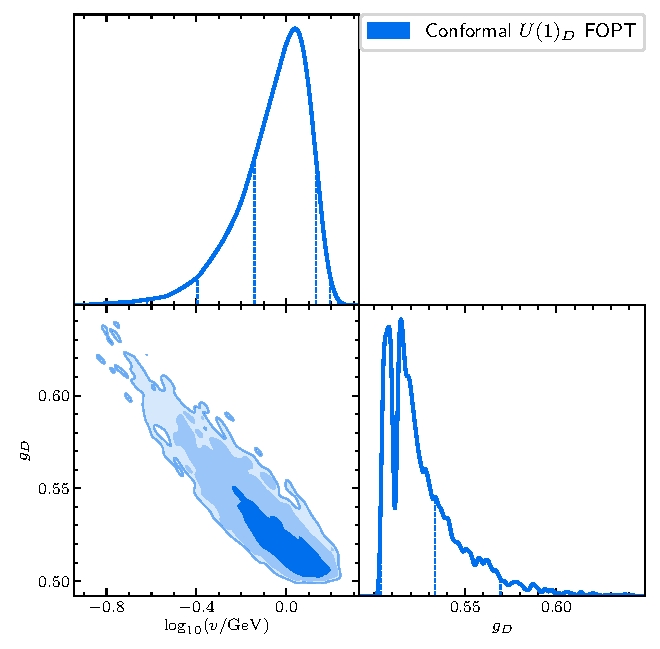
\includegraphics[width=0.70\textwidth]{u1conformal_posteriors.pdf}
\caption{Bayesian posterior distributions of $(\log_{10}v,\gD)$ from the
PTArcade NG15 \texttt{ceffyl} campaign
(source: \texttt{u1conformal\_posteriors.pdf}).}
\label{fig:posteriors}
\end{figure}

\section{Constraints}
\label{sec:constraints}
The \texttt{constraint-agent} evaluated 12 constraints on the PTArcade $1\sigma$
region ($\gD\in[0.508,0.546]$, $v\in[0.61,1.23]$~GeV; $\mAp\in[0.31,0.67]$~GeV,
$\mrho\in[10.7,24.4]$~MeV, $T_{\rm reh}\sim60$--$100$~MeV).
\textbf{No constraint excludes any part of the region.} Of the 12 constraints,
1 is directly testable, 2 approximately, 3 require recasting, 4 require new
backend calculations, and 2 are not applicable. A key physics point is that
$2\mrho\sim21$--$49$~MeV $\ll\mAp\sim0.3$--$0.7$~GeV, so the dark decay
$A'\to\rho\rho$ is kinematically open and can render $A'$ largely invisible to
visible-decay searches. SN1987A (C07) is \emph{not applicable} because the
preferred dark-photon mass lies above its $\lesssim100$~MeV reach. The central
internal tension flagged by the critic and constraint agents is that $\xi=1$
(which feeds $g_*$ and the GW redshift) requires a nonzero portal, whereas both
$\epsilon$ and $\lambda_{H\Phi}$ are set $\simeq0$ for the GW dynamics; this
gates most cosmological/laboratory bounds. The constraints are summarised in
Table~\ref{tab:constraints}.

\begin{longtable}{l p{0.32\textwidth} l l p{0.20\textwidth}}
\caption{Constraints on the $1\sigma$ region (source:
\texttt{handoff\_constraints.json}). Class: D=direct, A=approximate, R=recast,
N=new backend, NA=not applicable.}
\label{tab:constraints}\\
\toprule
ID & Constraint & Class & Verdict & Source \\
\midrule
\endfirsthead
\toprule
ID & Constraint & Class & Verdict & Source \\
\midrule
\endhead
C01 & BBN MeV-reheating ($T_{\rm reh}>3$~MeV) & D & allowed ($T_{\rm reh}\sim60$--$100$~MeV) & 2502.19478 \\
C02 & $\Delta N_{\rm eff}$ (dark radiation) & N & pending & 2502.19478 \\
C03 & Thermalization / $\xi=1$ justification & N & pending ($\epsilon_{\rm min}$) & 2502.19478 \\
C04 & Visible-decay collider ($A'$) & R & pending ($\epsilon$, BR) & 2603.08430 \\
C05 & Electron beam-dump (E137 etc.) & R & pending ($\epsilon$, $\tau$) & 1406.2698 \\
C06 & Invisible / missing-energy ($A'$) & R & pending ($\epsilon$, BR) & 2603.08430 \\
C07 & SN1987A energy loss & NA & not applicable ($\mAp>0.1$~GeV) & 1611.03864 \\
C08 & Scalon late decay (BBN/CMB) & N & pending ($\tau_\rho$, $Y_\rho$) & 2502.19478 \\
C09 & Scalon relic overabundance & N & pending ($\langle\sigma v\rangle$) & 2502.19478 \\
C10 & Higgs portal / $h\to$inv & A & allowed ($\lambda_{H\Phi}\ll10^{-10}$) & 2501.11619 \\
C11 & Perturbativity of $\gD$ & D & allowed ($\alpha_D\sim0.02$) & 1707.06765 \\
C12 & Dark-photon direct detection & NA & not applicable ($A'$ not DM) & 2603.08430 \\
\bottomrule
\end{longtable}

\paragraph{Missing backend calculations.} Four high-priority calculations gate
constraints C02--C09: (M1) minimum kinetic mixing $\epsilon$ for $\xi=1$
thermalization; (M2) dark-photon decay widths/lifetime and
$A'\to\rho\rho$ vs visible branching ratios; (M3) $\Delta N_{\rm eff}$ for the
thermalized MeV-scale dark sector; (M4) scalon relic yield, lifetime and
BBN/CMB energy injection.

\section{Assumptions and limitations}
\label{sec:assumptions}
The \texttt{prior-agent} audited 22 items (severity distribution peaks at 5;
four items at severity~8 and one at severity~9). The highest-severity and
uncontrolled items are collected in Table~\ref{tab:assumptions}. The three
dominant limiting factors are: (i)~the gauge-dependence theory uncertainty
(A07, order-of-magnitude on $\Ombg$); (ii)~the $\xi=1$ versus $\epsilon\simeq0$
internal tension (A05) and the associated cosmology calculations (A19, A20,
A21); and (iii)~the no-SMBHB-foreground PTArcade fit (A17), since NANOGrav
new-physics preferred regions depend strongly on astrophysical-foreground
modelling. Consequently \textbf{the preferred region is provisional}.

\begin{table}[ht]
\centering\small
\caption{High-severity ($\geq8$) and selected assumptions/limitations
(source: \texttt{handoff\_prior\_audit.json}). Ctrl=controlled.}
\label{tab:assumptions}
\begin{tabular}{l c c p{0.55\textwidth}}
\toprule
ID & Sev. & Ctrl & Description \\
\midrule
A19 & 9 & no & Four high-priority missing calculations gate C02--C09. \\
A05 & 8 & no & $\xi=1$ requires a portal, but $\epsilon,\lambda_{H\Phi}\simeq0$
(central internal tension). \\
A07 & 8 & no & Gauge dependence of CW+thermal $V_{\rm eff}$: order-of-magnitude
on $\Ombg$ (1707.06765). \\
A17 & 8 & no & Model-only (no SMBHB foreground) fit to NG15; preferred region
provisional. \\
A20 & 8 & no & Scalon (11--24~MeV) fate: overclosure (if stable) or late decay
(if $\epsilon\neq0$). \\
A03 & 7 & no & Kinetic mixing $\epsilon\simeq0$ for PT/GW; nonzero on cosmology
side. \\
A11 & 7 & yes & Very large $\alpha$ ($\sim10^{16}$); eternal-inflation/
percolation failures excluded. \\
A21 & 7 & no & $\Delta N_{\rm eff}$ likely strongest test of $\xi=1$. \\
A08 & 6 & no & No RG running / no daisy resummation ($\mu=v$). \\
A12 & 6 & yes & \texttt{dbf} template choice; higgsless out of domain. \\
A15 & 4 & yes & PTArcade priors; posterior interior, no boundary contact. \\
\bottomrule
\end{tabular}
\end{table}

\section{Conclusions}
\label{sec:conclusions}
The classically scale-invariant dark $U(1)_D$ model with CW radiative breaking
produces a strongly supercooled FOPT whose SGWB falls in the nHz band probed by
PTAs. A PTArcade NG15 campaign with the physically motivated \texttt{dbf}
template prefers $v\simeq1.09$~GeV, $\gD\simeq0.528$ (MAP), i.e.\ a GeV-scale
dark photon and an MeV-scale scalon, in line with the literature scale for this
model class~\cite{Goncalves2025,Balan2025}.

\textbf{Robust:} the model is theoretically consistent (no anomalies, correct
dof bookkeeping, perturbative $\gD$, C11); the FOPT is strongly supercooled and
lands in the nHz band; the \texttt{dbf} template is the correct strong-supercooling
choice; the BBN reheating floor (C01) and Higgs-portal/perturbativity bounds
(C10, C11) are satisfied; SN1987A and dark-photon direct detection are not
applicable (C07, C12).

\textbf{Conditional / provisional:} the preferred region depends on the no-SMBHB
fit (A17) and carries an order-of-magnitude gauge-dependence uncertainty (A07);
no constraint currently excludes it, but most cosmological/laboratory bounds are
not yet applicable.

\textbf{Blocked / uncontrolled:} the $\xi=1$ versus $\epsilon\simeq0$ tension
(A05) and the four missing calculations (A19; $\epsilon_{\rm min}$,
$A'$ branchings, $\Delta N_{\rm eff}$, scalon relic/decay) must be resolved
before the viability of the region can be confirmed. Recommended follow-ups
include refitting with an SMBHB foreground, propagating a gauge-variation band,
and running the four dark-sector cosmology modules.

\section{Inconsistencies}
\label{sec:inconsistencies}
No contradictory numerical claims were found across handoffs. One physics-level
internal tension is propagated consistently by all agents and is \emph{not}
silently resolved here: $\xi=1$ (used by the FOPT/PTA stages to set $g_*$ and
the GW redshift) is incompatible with exactly vanishing portals
($\epsilon=\lambda_{H\Phi}=0$); a minimum nonzero $\epsilon$ is required and
remains to be computed (A05, C03).

\begin{thebibliography}{9}
\bibitem{Goncalves2025} J.~Gon\c{c}alves, D.~Marfatia, A.~P.~Morais,
R.~Pasechnik, \emph{Supercooled phase transitions in conformal dark sectors
explain NANOGrav data}, Phys.\ Lett.\ B \textbf{869} (2025) 139829,
arXiv:2501.11619.
\bibitem{Balan2025} S.~Balan, T.~Bringmann, F.~Kahlhoefer, J.~Matuszak,
C.~Tasillo, \emph{Sub-GeV dark matter and nano-Hertz gravitational waves from a
classically conformal dark sector}, JCAP \textbf{08} (2025) 062,
arXiv:2502.19478.
\bibitem{Fujikura2023} K.~Fujikura, S.~Girmohanta, Y.~Nakai, M.~Suzuki,
\emph{NANOGrav Signal from a Dark Conformal Phase Transition},
Phys.\ Lett.\ B (2023), arXiv:2306.17086.
\bibitem{Borah2021} D.~Borah, A.~Dasgupta, S.~K.~Kang, \emph{Gravitational waves
from a dark $U(1)_D$ phase transition in light of NANOGrav 12.5 yr data},
Phys.\ Rev.\ D \textbf{104} (2021) 063501, arXiv:2105.01007.
\bibitem{Mohamadnejad2020} A.~Mohamadnejad, \emph{Gravitational waves from
scale-invariant vector dark matter model: Probing below the neutrino-floor},
Eur.\ Phys.\ J.\ C \textbf{80} (2020) 197, arXiv:1907.08899.
\bibitem{Feng2026} W.-Z.~Feng, Z.-H.~Zhang, \emph{Gauge-independent gravitational
waves from a minimal dark $U(1)$ sector with viable dark matter candidates},
arXiv:2602.14866.
\bibitem{Chiang2017} C.-W.~Chiang, E.~Senaha, \emph{On gauge dependence of
gravitational waves from a first-order phase transition in classical
scale-invariant $U(1)'$ models}, Phys.\ Lett.\ B \textbf{774} (2017) 489,
arXiv:1707.06765.
\bibitem{Lewicki2025} M.~Lewicki, V.~Vaskonen, \emph{Impact of cosmic expansion
on gravitational wave spectra from strongly supercooled first-order phase
transitions}, arXiv:2511.15687.
\bibitem{Jinno2022} R.~Jinno, T.~Konstandin, H.~Rubira, I.~Stomberg,
\emph{Higgsless simulations of cosmological phase transitions and gravitational
waves}, JCAP \textbf{02} (2023) 011, arXiv:2209.04369.
\bibitem{Batell2014} B.~Batell, R.~Essig, Z.~Surujon, \emph{Strong Constraints
on Sub-GeV Dark Sectors from SLAC Beam Dump E137}, Phys.\ Rev.\ Lett.\
\textbf{113} (2014) 171802, arXiv:1406.2698.
\bibitem{Chang2017} J.~H.~Chang, R.~Essig, S.~D.~McDermott, \emph{Revisiting
Supernova 1987A Constraints on Dark Photons}, JHEP \textbf{01} (2017) 107,
arXiv:1611.03864.
\bibitem{Caputo2026} A.~Caputo, R.~Essig, \emph{The Dark Photon: a 2026
Perspective}, arXiv:2603.08430.
\end{thebibliography}

\end{document}
